

%\renewcommand{\lastmod}{April 29, 2020}

\chapter{Zweiatomige Kette dargestellt als einatomig}



\paragraph{Einatomige  Kette} Masse $M$, Gitterkonstante $a_1$, Federkonstante $c$


\begin{equation}
\omega = \sqrt{\frac{4 \, c}{M}} \left| \sin \left(\frac{1}{2} \,  k \, a_1  \right) \right|
\end{equation}




\paragraph{Zweiatomige  Kette}  Gitterkonstante $a_2$, Federkonstante $c$, Massen $M_1$, $M_2$ und reduzierte Masse $\mu = M_1 M_2 / (M_1 + M_2)$

\begin{equation}
\omega^2 =  \frac{c}{\mu}
\pm c \sqrt{ \frac{1}{\mu^2} - \frac{4}{M_1 M_2}  \sin^2 \left( \frac{1}{2}  k \, a_2 \right) } 
\end{equation}

Annahme: beide Massen identisch, also $M_1 = M_2 = M$ und damit $\mu = M/2$, und $a_2 = 2 a_1$
\begin{align}
\omega^2 =  & \frac{2c}{M}
\pm c \sqrt{ \frac{4}{M^2} - \frac{4}{M^2}  \sin^2 \left( \frac{1}{2}  k \, a_2 \right) }  \\
= &\frac{2c}{M}
\pm \frac{2c}{M} \sqrt{ 1 -   \sin^2 \left( \frac{1}{2}  k \, a_2 \right) }  \\
= &\frac{2c}{M}
\pm \frac{2c}{M}   \cos \left( \frac{1}{2}  k \, a_2 \right)   \\
= &\frac{2c}{M} \left( 1 
\pm   \cos \left(   k \, a_1 \right)    \right)
\end{align}

Zuerst den Minus-Zweig (mit $\sin(x/2) = \sqrt{ 1-\cos(x) } / \sqrt{2}$)
\begin{align}
\omega_{-} =  & \sqrt{\frac{2c}{M}} \, \sqrt{1 - 
  \cos \left(   k \, a_1 \right) }  \\
=  & \sqrt{\frac{4c}{M}} \, 
  \sin \left( \frac{1}{2}   k \, a_1 \right) 
\end{align}
stimmt also mit einatomiger Kette überein (zzgl. Betrag wegen Wurzel-Ziehen)

Jetzt plus-Zweig (mit $\cos(x/2) = \sqrt{ 1+\cos(x) } / \sqrt{2}$)
\begin{align}
\omega_{+} =  & \sqrt{\frac{2c}{M}} \, \sqrt{1 + 
  \cos \left(   k \, a_1 \right) }  \\
=  & \sqrt{\frac{4c}{M}} \, 
  \cos \left( \frac{1}{2}   k \, a_1 \right)  \\
  =  & \sqrt{\frac{4c}{M}} \, 
  \sin \left( \frac{1}{2}   k \, a_1 + \frac{\pi}{2} \right)  \\
    =  & \sqrt{\frac{4c}{M}} \, 
  \sin \left( \frac{1}{2}   (k + G)  \, a_1 \right) 
\end{align}
mit $G   =\pi / a_1 = 2 \pi / a_2$, also dem kürzesten reziproken Gittervektor der \emph{zweiatomigen} Kette. Auch optischer Ast stimmt mit einatomiger Kette überein, ist aber um $G$ verschoben (zzgl. Betrag wegen Wurzel-Ziehen).




  \begin{figure}
  


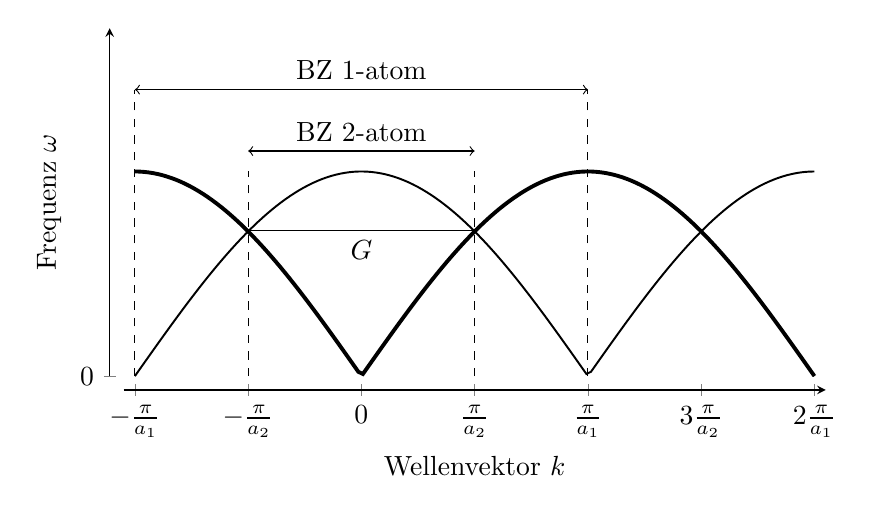
\begin{tikzpicture}[
declare function={ 
   m1 = 1;
   m2 = 1;
   mu = (m1 * m2) / (m1 + m2);
   omp(\x) = ( 1/mu ) + sqrt( (1 / mu^2) - (4 / (m1 * m2))  * sin(\x) ^2);
   omm(\x) = ( 1/mu ) - sqrt( (1 / mu^2) - (4 / (m1 * m2))  * sin(\x) ^2);   
      %omp(\x) =  1 + sin(x) ;
	  },
]

%\omega^2 =  \frac{c}{\mu}
%\pm c \sqrt{ \frac{1}{\mu^2} - \frac{4}{M_1 M_2}  \sin^2 \left( %\frac{1}{2}  \mathbf{k} \cdot \mathbf{a} \right) } 


%\useasboundingbox (0,0) rectangle (5,5);
%\draw (0,0) rectangle (5,5);

\begin{axis}[no markers, 
	samples=150,
    %      ymin=-0.3, ymax=1,
     xmin = -2.1, xmax = 4.1,
    ymin = 0, ymax = 1.7,
      %  axis y line=left,
       %    axis x line=bottom,
         xtick = {-2, -1, 0,1,2, 3, 4},
          xticklabels= {$-\frac{\pi}{a_1}$,$-\frac{\pi}{a_2}$, 0, $\frac{\pi}{a_2}$, $\frac{\pi}{a_1}$, $3 \frac{\pi}{a_2}$, $2 \frac{\pi}{a_1}$ },
ytick = {0},
            xlabel = {Wellenvektor $k$ },
        ylabel = {Frequenz $\omega$},    
        %x label style={at={(axis description cs:1, 0)},anchor=north east, yshift=-7pt},
    %y label style={at={(axis description cs: 0,1)},anchor=south east,  yshift=10pt},
           width= 10.5cm, height = 6cm,
  separate axis lines,
  axis x line=bottom,
  axis x line shift=5pt,
  %xlabel shift=10pt,
  axis y line=left,
  axis y line shift=5pt,
%  ylabel shift=10pt           
           ]
           
\addplot [domain=-2:4,  line width=1.4pt]    {abs(sin(x * 45) ) };
\addplot [domain=-2:4,  line width=0.7pt]    {abs(sin(x * 45 + 90) ) };
 
\draw[->] (-1, 0.71) -- node[below]{$G$} (1,0.71); 
 
\draw[dashed] (-1,0) -- (-1, 1);  
\draw[dashed] (1,0) -- (1, 1);  
\draw[<->] (-1, 1.1) --node[above]{BZ 2-atom}  (1, 1.1);
 
 \draw[dashed] (-2,0) -- (-2, 1.4);  
\draw[dashed] (2,0) -- (2, 1.4);  
\draw[<->] (-2, 1.4) --node[above]{BZ 1-atom}  (2, 1.4);


 
 
%\node[anchor = north] at (0.5, 0.5) {\footnotesize akustisch} ;
%\node[anchor = north] at (0.3, 1.75) {\footnotesize optisch} ;
 
 
 \end{axis}

\end{tikzpicture}

\caption{Dispersionsrelationen ein- und zweiatomiger Ketten identischer Massen.}
  \end{figure}

Die Dispersionsrelation der zweiatomigen Kette mit identischen Massen entsteht aus der einatomigen, indem man diese an der Grenze der BZ der zweiatomigen \emph{zurückfaltet}. Dies spielt eine wichtige Rolle bei der Dispersionsrelation von Elektronen im Gitter (engl: folded zone scheme). Schon die Annahme eines Gitters hat einen Einfluss auf die Dispersionsrelation. Wenn man die einatomige Kette als zweiatomig betrachtet, nimmt man an, dass etwas periodisch in $a_2 = 2 a_1$ ist. Man nimmt also ein Gitter an, das über dem einatomigen liegt. Es spielt dabei keine Rolle, dass es 'leer' ist, also sich nichts mit $a_2$ ändert. Bei den Elektronen wird dies 'empty lattice approximation' genannt und führt zur Bandlücke der Elektronen im Festkörper.



%-------------------

